% Provenance (never printed): cycle 4 SVT, "La planete Terre, l'environnement
% et l'action humaine": natural risks, hazard and vulnerability, prevention
% and protection; see sources/book1/PROVENANCE.md. Book 1, grade 9, chapter 2.
% Vocabulary guard: owns risk, vulnerability, prevention, hazard map.
% Natural hazard and natural disaster, the warning colours and the safety
% rules are g5's (natural-hazards); the warning signs of an eruption and the
% Pinatubo story are g7's (volcanoes); seismometer, tsunami and "scientists
% cannot predict earthquakes" are g7's (earthquakes); flood and floodplain
% are g5's (water-shapes-the-land); weather forecast is g8's. Lahars are
% called mudflows (as in g7). "Normal fault" is Book 2's: here "a fault".
\chapter{Leven met natuurrisico's}\label{ch:g9:natural-risks}

Laat in de avond van 13~november 1985 lagen de meeste inwoners van
Armero, een stad in Colombia, in bed. Een \omterm{def:g5:natural-hazards:storm}{storm} verborg de besneeuwde
\omterm{def:g4:volcanoes-earthquakes-first-look:volcano}{vulkaan} Nevado del Ruiz, \qty{45}{km} verderop, en niemand in de stad zag
hem uitbarsten. Het hete \omterm{def:g3:stones-pebbles-sand:rock}{gesteente} smolt een deel van zijn ijs, en het
water, vermengd met as en \omterm{def:g3:stones-pebbles-sand:rock}{gesteente}, stortte als modderstromen door de
\omterm{def:g1:landscapes-around-us:landform}{dalen} naar beneden. Ongeveer twee uur later stroomden de modderstromen
uit het \omterm{def:g1:landscapes-around-us:landform}{dal} van de \omterm{def:g1:landscapes-around-us:water}{rivier} de Lagunillas, recht de stad in: zo'n
\num{23000} mensen, het grootste deel van de stad, kwamen om. Twee uur was
genoeg tijd om naar hoger gelegen grond te lopen. De inwoners van Armero
werden niet gewaarschuwd.
% ledger: usgs:armero

\begin{omfigure}
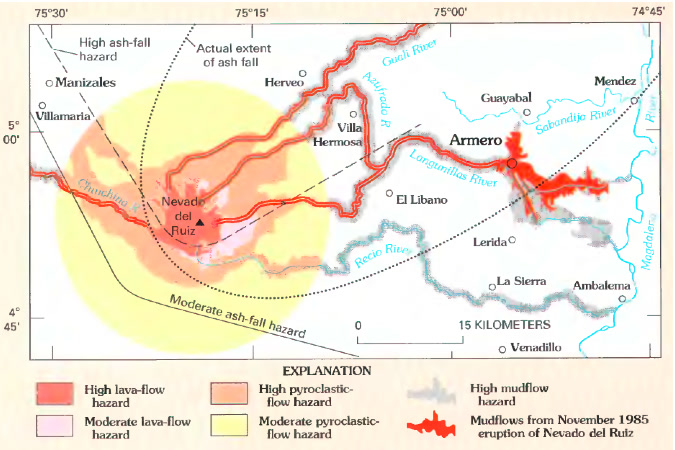
\includegraphics[width=0.86\linewidth]{images/book1/g9-ruiz-hazard-map.jpg}

{\small De \omterm{def:g9:natural-risks:hazard-map}{gevarenkaart} van de Nevado del Ruiz. Een eerste versie,
getekend door Colombiaanse geologen, deed een maand voor de \omterm{def:g4:volcanoes-earthquakes-first-look:eruption}{uitbarsting}
de ronde en toonde al het gevaar van modderstromen in het \omterm{def:g1:landscapes-around-us:landform}{dal} van Armero.
Deze versie, na de ramp opnieuw getekend, voegt in felrood de
modderstromen toe die in november 1985 werkelijk kwamen (de gearceerde
cirkel rond de \omterm{def:g4:volcanoes-earthquakes-first-look:volcano}{vulkaan} heeft een straal van ongeveer \qty{20}{km}). Naar
T.~L.~Wright en T.~C.~Pierson, USGS Circular 1073, 1992 (publiek domein, via
Wikimedia Commons).}
% ledger: usgs:ruiz-map, commons:ruiz-map
\label{fig:g9:natural-risks:ruiz}
\end{omfigure}

Zes jaar later werd de Pinatubo in de Filipijnen in de gaten gehouden,
kwam de waarschuwing op tijd en vertrokken de mensen
(\cref{ch:g7:volcanoes}). Het waren allebei explosieve \omterm{def:g4:volcanoes-earthquakes-first-look:volcano}{vulkanen}, met
mensen die op de route van hun modderstromen woonden. Wat verschilde, was
wat de mensen wisten, en wat ze ermee deden. Dit hoofdstuk gaat over dat
verschil.
% ledger: usgs:armero (Pinatubo 1991 averted a disaster like Armero), usgs:pinatubo-1991

\begin{recall}
Een \emph{\omterm{def:g5:natural-hazards:hazard}{natuurgevaar}} is een natuurlijke gebeurtenis die mensen schade
kan toebrengen; het wordt een \emph{\omterm{def:g5:natural-hazards:disaster}{natuurramp}} als het toeslaat waar
mensen wonen en grote schade aanricht (\cref{ch:g5:natural-hazards}). Een
\omterm{def:g1:landscapes-around-us:water}{rivier} die buiten haar oevers treedt, bedekt haar \omterm{def:g5:water-shapes-the-land:flood}{overstromingsvlakte}
(\cref{ch:g5:water-shapes-the-land}). Een \omterm{def:g4:volcanoes-earthquakes-first-look:volcano}{vulkaan} geeft voor een grote
\omterm{def:g4:volcanoes-earthquakes-first-look:eruption}{uitbarsting} vaak waarschuwingssignalen: kleine \omterm{def:g4:volcanoes-earthquakes-first-look:earthquake}{aardbevingen}, zwellende
hellingen, gas (\cref{ch:g7:volcanoes}). Wetenschappers kunnen
\omterm{def:g4:volcanoes-earthquakes-first-look:earthquake}{aardbevingen} niet voorspellen; \omterm{def:g7:earthquakes:seismometer}{seismometers} registreren ze, en een
\omterm{def:g4:volcanoes-earthquakes-first-look:earthquake}{aardbeving} onder de \omterm{def:g2:water-on-earth:ocean}{zee} kan een \omterm{def:g7:earthquakes:tsunami}{tsunami} veroorzaken
(\cref{ch:g7:earthquakes}). Een \omterm{def:g8:fronts-and-weather-maps:forecast}{weersverwachting} zegt wat voor \omterm{def:g1:watching-the-weather:weather}{weer} het de
komende dagen wordt (\cref{ch:g8:fronts-and-weather-maps}).
\end{recall}

\section{Gevaar, kwetsbaarheid en risico}

Dezelfde \omterm{def:g4:volcanoes-earthquakes-first-look:earthquake}{aardbeving} richt niet overal dezelfde schade aan. Onder een lege
\omterm{def:g5:weather-and-climate:desert}{woestijn} treft ze niemand. Onder een stad met stevige gebouwen, waarvan de
inwoners weten wat ze moeten doen, schudt ze, maakt ze mensen bang en
breekt ze ruiten. Onder een stad met zware, slecht gebouwde huizen kan ze
die op de mensen binnen laten instorten. Het gevaar is hetzelfde; wat
verandert, is hoe gemakkelijk de plaats schade kan oplopen.

\begin{definition}[Kwetsbaarheid]\label{def:g9:natural-risks:vulnerability}
De \emph{kwetsbaarheid}\index{kwetsbaarheid} van een plaats is hoe
gemakkelijk haar inwoners, haar gebouwen en de dingen die ze nodig hebben
door een \omterm{def:g5:natural-hazards:hazard}{natuurgevaar} schade kunnen oplopen. Woningen op een
\omterm{def:g5:water-shapes-the-land:flood}{overstromingsvlakte}, zwakke gebouwen, geen waarschuwing en geen plan
maken een plaats kwetsbaar.
\end{definition}

\begin{definition}[Risico]\label{def:g9:natural-risks:risk}
Het \emph{risico}\index{risico} dat een plaats door een \omterm{def:g5:natural-hazards:hazard}{natuurgevaar} loopt,
is het gevaar dat haar inwoners en hun bezittingen schade oplopen. Het
hangt zowel af van het gevaar, hoe sterk en hoe vaak het is, als van de
\omterm{def:g9:natural-risks:vulnerability}{kwetsbaarheid} van de plaats: waar geen gevaar is, of niets dat schade kan
oplopen, is er geen risico.
\end{definition}

\begin{omfigure}
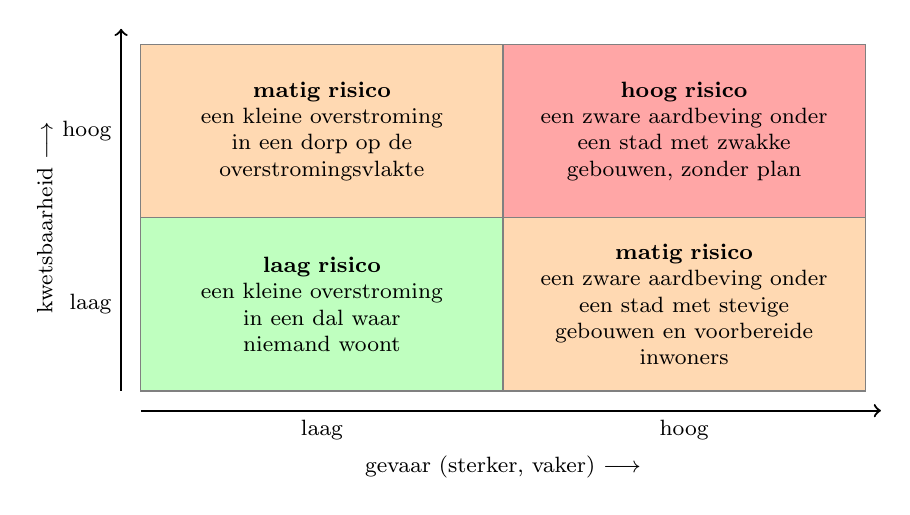
\begin{tikzpicture}[x=1cm, y=1cm, font=\footnotesize,
    cell/.style={minimum width=4.6cm, minimum height=2.2cm, align=center, draw=black!50, text width=4.2cm}]
  \node[cell, fill=green!25] at (2.3,1.1) {\textbf{laag risico}\\ een kleine overstroming\\ in een dal waar\\ niemand woont};
  \node[cell, fill=orange!30] at (6.9,1.1) {\textbf{matig risico}\\ een zware aardbeving onder\\ een stad met stevige\\ gebouwen en voorbereide\\ inwoners};
  \node[cell, fill=orange!30] at (2.3,3.3) {\textbf{matig risico}\\ een kleine overstroming\\ in een dorp op de\\ overstromingsvlakte};
  \node[cell, fill=red!35] at (6.9,3.3) {\textbf{hoog risico}\\ een zware aardbeving onder\\ een stad met zwakke\\ gebouwen, zonder plan};
  \draw[->, thick] (0,-0.25) -- (9.4,-0.25);
  \draw[->, thick] (-0.25,0) -- (-0.25,4.6);
  \node[anchor=north] at (4.6,-0.7) {gevaar (sterker, vaker) $\longrightarrow$};
  \node[rotate=90, anchor=south] at (-1.0,2.2) {kwetsbaarheid $\longrightarrow$};
  \node[below] at (2.3,-0.25) {laag};
  \node[below] at (6.9,-0.25) {hoog};
  \node[left] at (-0.25,1.1) {laag};
  \node[left] at (-0.25,3.3) {hoog};
\end{tikzpicture}

{\small Het risicorooster (een schets). Het \omterm{def:g9:natural-risks:risk}{risico} groeit met het gevaar
en met de \omterm{def:g9:natural-risks:vulnerability}{kwetsbaarheid}. Een stad verplaatsen is zelden mogelijk, en een
gevaar kun je niet uitzetten; maar de \omterm{def:g9:natural-risks:vulnerability}{kwetsbaarheid} kan omlaag, en dat
brengt de stad lager in het rooster.}
\label{fig:g9:natural-risks:grid}
\end{omfigure}

Armero was een plaats met een groot gevaar: een besneeuwde \omterm{def:g4:volcanoes-earthquakes-first-look:volcano}{vulkaan} die
een jaar eerder was ontwaakt, en een stad gebouwd op de afzettingen van
oude modderstromen, aan de \omterm{def:g5:water-shapes-the-land:source-mouth}{monding} van een \omterm{def:g1:landscapes-around-us:landform}{dal} dat ze al eerder had
aangevoerd. Ze was ook zeer kwetsbaar: de wetenschappers hadden te weinig
instrumenten en steun, de informatie aan de autoriteiten was vaak vaag, en
er bestond geen evacuatieplan en geen snelle manier om de stad te
waarschuwen.
% ledger: usgs:armero

\section{Voorspellen en voorkomen}

Sommige gevaren zie je aankomen. Een \omterm{def:g5:natural-hazards:storm}{storm} wordt dagen van tevoren
voorspeld (\cref{ch:g8:fronts-and-weather-maps}); een \omterm{def:g5:water-shapes-the-land:flood}{overstroming} na
zware \omterm{def:g4:clouds-rain-snow:precipitation}{regen} uren tot dagen van tevoren; een grote \omterm{def:g4:volcanoes-earthquakes-first-look:eruption}{uitbarsting} kondigt
zich vaak dagen tot weken van tevoren aan, maar niet altijd. Een \omterm{def:g7:earthquakes:tsunami}{tsunami}
steekt een \omterm{def:g2:water-on-earth:ocean}{oceaan} in uren over, zodat een waarschuwing verre \omterm{def:g1:landscapes-around-us:water}{kusten} kan
bereiken voordat hij dat doet. \omterm{def:g4:volcanoes-earthquakes-first-look:earthquake}{Aardbevingen} daarentegen kunnen niet worden
voorspeld: wetenschappers kunnen zeggen welke \omterm{def:g7:earthquakes:fault}{breuken} op een dag opnieuw
zullen verschuiven, nooit op welke dag.
% ledger: nws:tsunami-speed, usgs:eq-basics, usgs:pinatubo-1991

Een voorspelling, hoe goed ook, is alleen nuttig als er iets wordt gedaan
voordat het gevaar toeslaat. Het meeste van dat werk gebeurt lang voor
elke waarschuwing.

\begin{definition}[Preventie]\label{def:g9:natural-risks:prevention}
\emph{Preventie}\index{preventie} is alles wat wordt gedaan voordat een
\omterm{def:g5:natural-hazards:hazard}{natuurgevaar} toeslaat om het \omterm{def:g9:natural-risks:risk}{risico} te verlagen: weten waar het gevaar kan
toeslaan, op veilige plaatsen en op veilige manieren bouwen, het gevaar in
de gaten houden, mensen waarschuwen en ze voorbereiden.
\end{definition}

\omterm{def:g9:natural-risks:prevention}{Preventie} werkt aan beide kanten van het risicorooster. Een \omterm{def:g4:volcanoes-earthquakes-first-look:volcano}{vulkaan} of
een \omterm{def:g1:landscapes-around-us:water}{rivier} in de gaten houden maakt hem niet minder gevaarlijk, maar geeft
tijd om te handelen. Weg van de \omterm{def:g5:water-shapes-the-land:flood}{overstromingsvlakte} bouwen, stevige
huizen bouwen, de routes naar hoger gelegen grond plannen en ze oefenen:
dat alles verlaagt de \omterm{def:g9:natural-risks:vulnerability}{kwetsbaarheid}.

\begin{omfigure}
\begin{minipage}[c]{0.44\linewidth}\centering
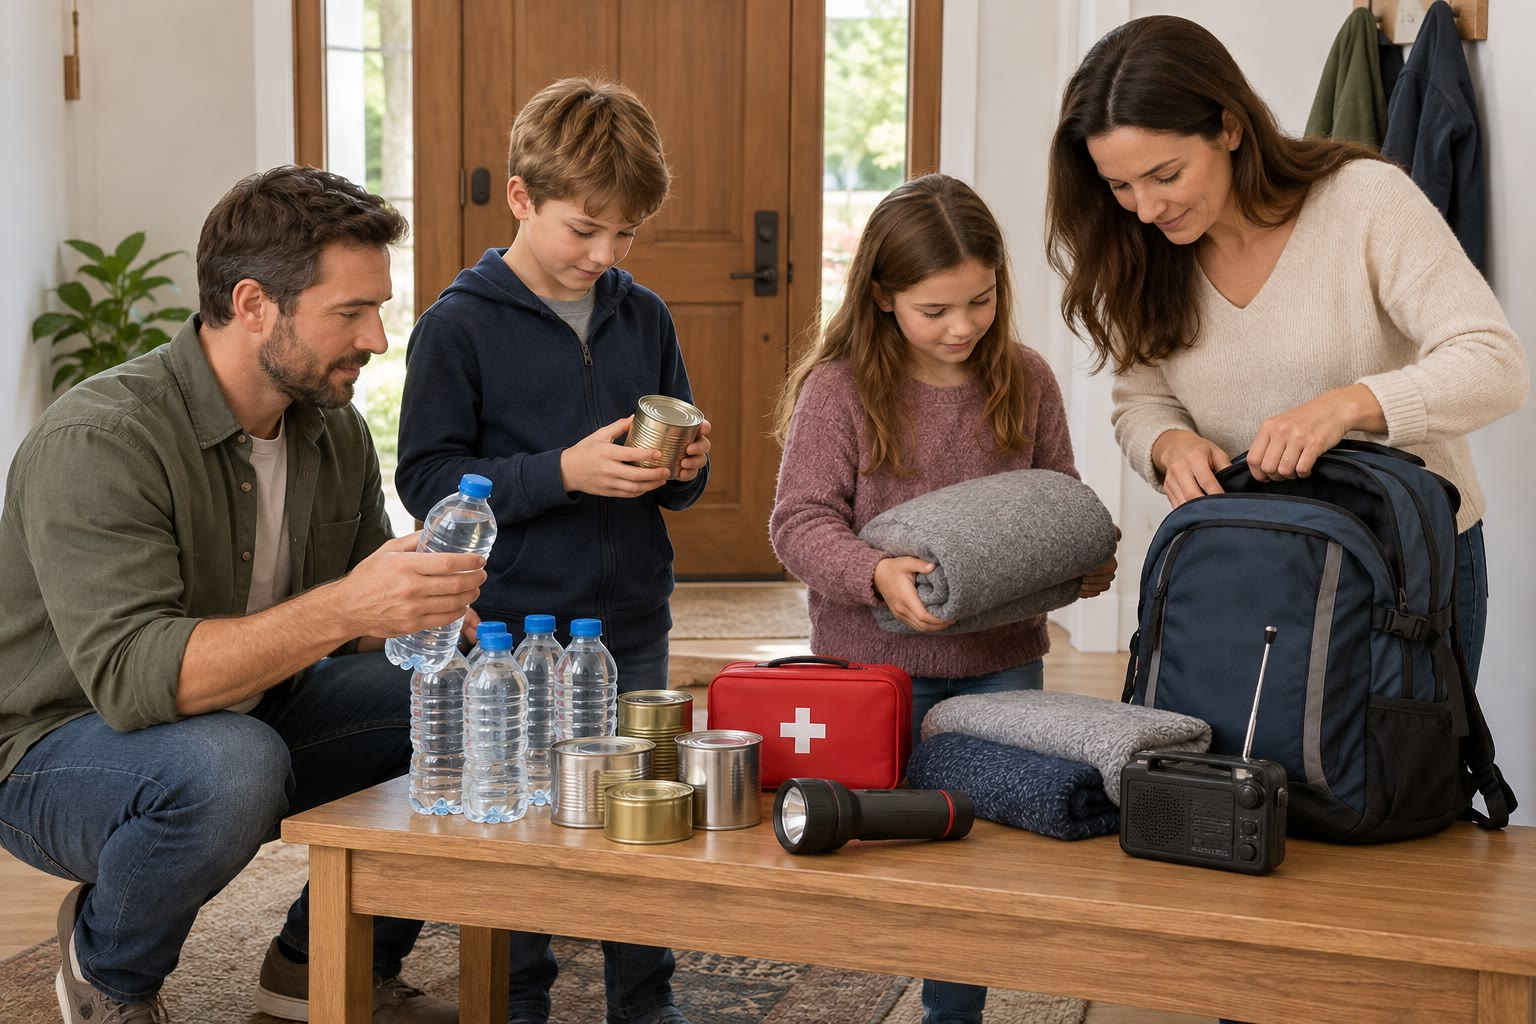
\includegraphics[width=\linewidth]{images/book1/ai/g9-emergency-kit.jpg}
\end{minipage}\hfill
\begin{minipage}[c]{0.52\linewidth}\raggedright
{\small Voorbereid zijn: een gezin controleert zijn noodpakket, dat bij
de deur ligt, klaar om mee te nemen als ze snel weg moeten: water en
voedsel dat een paar dagen houdbaar is, een zaklamp, een radio die zonder
stroom uit het stopcontact werkt, reservebatterijen, een EHBO-doos en
warme dekens (door AI gegenereerde illustratie van een algemene scène).}
\end{minipage}
% ledger: ready:kit
\label{fig:g9:natural-risks:kit}
\end{omfigure}

\section{Vulkanen en breuken in de gaten houden}

Een vulkanologisch observatorium houdt de waarschuwingssignalen van
\cref{ch:g7:volcanoes} in de gaten met instrumenten die dag en nacht
werken en hun metingen naar het observatorium sturen.
% ledger: usgs:hvo-toolkit

\begin{omfigure}
\begin{tikzpicture}[x=1cm, y=1cm, font=\footnotesize, >={Stealth[length=2mm]}]
  % ground and cone
  \fill[black!13] (0,0) -- (0,1.0) -- (3.0,1.2) -- (5.4,3.6) -- (6.4,3.6) -- (8.8,1.2) -- (12,1.0) -- (12,0) -- cycle;
  \draw[black!60] (0,1.0) -- (3.0,1.2) -- (5.4,3.6) -- (6.4,3.6) -- (8.8,1.2) -- (12,1.0);
  % magma chamber and conduit
  \fill[omWarm!70] (5.9,0.6) ellipse (1.5 and 0.38);
  \fill[omWarm!70] (5.75,0.9) rectangle (6.05,3.6);
  \node[white, font=\scriptsize\bfseries] at (5.9,0.58) {magma};
  % gas plume, drifting west
  \fill[black!10] (5.8,3.95) circle (0.3) (5.35,4.35) circle (0.4) (4.75,4.75) circle (0.45);
  % swollen east flank, dashed
  \draw[dashed, omWarm, line width=0.8pt] (6.45,3.7) .. controls (7.5,3.55) and (8.6,2.6) .. (8.85,1.25);
  \draw[->, omWarm] (7.3,2.75) -- (7.7,3.15);
  \node[anchor=west, align=left, text=omWarm!80!black] at (8.2,3.75) {opstijgend magma\\ doet de helling zwellen};
  % tiltmeter on the east flank
  \fill[black] (7.75,2.12) rectangle (8.05,2.24);
  \draw[black!70] (8.1,2.2) -- (8.5,2.45);
  \node[anchor=west, align=left] at (8.5,2.55) {hellingmeter: de helling\\ kantelt als ze zwelt};
  % GPS receiver on the west flank, and its satellite
  \draw[black, line width=0.6pt] (4.4,2.6) -- (4.4,2.95);
  \fill[black] (4.25,2.95) rectangle (4.55,3.05);
  \draw[black] (4.4,3.05) circle (0.1);
  \draw[black, fill=white] (1.7,4.85) rectangle (2.0,5.05);
  \draw[black] (1.4,4.95) -- (2.3,4.95);
  \node[anchor=east] at (1.35,4.95) {satelliet};
  \draw[black!50, dashed] (4.3,3.15) -- (2.05,4.8);
  \draw[black!70] (3.05,2.65) -- (4.2,2.85);
  \node[anchor=east, align=right] at (3.0,2.6) {gps-ontvanger: de\\ grond beweegt\\ millimeters};
  % gas instrument on the crater rim
  \fill[black] (6.45,3.6) rectangle (6.75,3.75);
  \draw[black!70] (6.8,3.75) -- (7.1,4.45);
  \node[anchor=west, align=left] at (7.1,4.6) {gasmeter: de gassen die\\ uit de krater ontsnappen};
  % seismometer (in the ground)
  \fill[black] (2.1,0.95) rectangle (2.4,1.1);
  \node[anchor=north, align=center] at (1.6,0.85) {seismometer:\\ kleine aardbevingen};
  % camera, east, looking at the summit
  \fill[black] (10.7,1.12) rectangle (11.0,1.32);
  \fill[black] (10.7,1.17) -- (10.55,1.12) -- (10.55,1.32) -- (10.7,1.27) -- cycle;
  \node[anchor=north, align=center] at (10.8,0.85) {camera:\\ bewaakt de top};
\end{tikzpicture}

{\small Een \omterm{def:g4:volcanoes-earthquakes-first-look:volcano}{vulkaan} in de gaten houden (een schets, niet op schaal).
\omterm{def:g7:earthquakes:seismometer}{Seismometers} tellen de kleine \omterm{def:g4:volcanoes-earthquakes-first-look:earthquake}{aardbevingen}; hellingmeters en
gps-ontvangers, vastgezet op de rots, meten hoe de grond kantelt en
beweegt terwijl er eronder \omterm{def:g7:volcanoes:magma}{magma} samenkomt; andere instrumenten meten de
gassen die ontsnappen; camera's bewaken de top. \omterm{def:g4:clouds-rain-snow:rain-gauge}{Regenmeters} helpen om de
signalen van de \omterm{def:g4:volcanoes-earthquakes-first-look:volcano}{vulkaan} te onderscheiden van de gevolgen van zware \omterm{def:g4:clouds-rain-snow:precipitation}{regen}.}
% ledger: usgs:hvo-toolkit
\label{fig:g9:natural-risks:monitoring}
\end{omfigure}

Geen van deze signalen geeft de dag en het uur van een \omterm{def:g4:volcanoes-earthquakes-first-look:eruption}{uitbarsting}. De
wetenschappers lezen ze samen, zoals een arts verscheidene metingen van
een patiënt leest, en zeggen hoe het gevaar verandert; de autoriteiten
beslissen wanneer een gebied wordt afgesloten en wanneer mensen worden
geëvacueerd. Bij de Pinatubo werkte deze keten. Bij de Nevado del Ruiz had
de \omterm{def:g4:volcanoes-earthquakes-first-look:volcano}{vulkaan} een jaar lang signalen gegeven, met zwermen \omterm{def:g4:volcanoes-earthquakes-first-look:earthquake}{aardbevingen}, maar
er waren weinig instrumenten, en de keten van de wetenschappers naar de
inwoners van Armero was verbroken.
% ledger: usgs:armero, usgs:hvo-toolkit, usgs:pinatubo-1991

\omterm{def:g7:earthquakes:fault}{Breuken} worden op dezelfde manier in de gaten gehouden, door netwerken van
\omterm{def:g7:earthquakes:seismometer}{seismometers} en van gps-stations die millimeter voor millimeter meten hoe
de twee kanten van een \omterm{def:g7:earthquakes:fault}{breuk} langzaam bewegen. Zo weet men welke \omterm{def:g7:earthquakes:fault}{breuken}
de spanning voor de volgende zware \omterm{def:g4:volcanoes-earthquakes-first-look:earthquake}{aardbeving} opbouwen, maar niet wanneer
die komt. Bij \omterm{def:g4:volcanoes-earthquakes-first-look:earthquake}{aardbevingen} is \omterm{def:g9:natural-risks:prevention}{preventie} de belangrijkste verdediging.
% ledger: usgs:gps, usgs:eq-basics

\section{Gevarenkaarten en overstromingszones}

De eerste stap van \omterm{def:g9:natural-risks:prevention}{preventie} is weten waar een gevaar kan toeslaan.

\begin{definition}[Gevarenkaart]\label{def:g9:natural-risks:hazard-map}
Een \emph{gevarenkaart}\index{gevarenkaart} toont de plaatsen die een
\omterm{def:g5:natural-hazards:hazard}{natuurgevaar} kan bereiken, vaak met verscheidene niveaus van gevaar. Ze
wordt getekend op basis van wat het gevaar in het verleden heeft gedaan en
van de vorm van het terrein.
\end{definition}

De \omterm{def:g2:drawing-to-map:map}{kaart} van de Nevado del Ruiz, aan het begin van dit hoofdstuk, is een
\omterm{def:g9:natural-risks:hazard-map}{gevarenkaart}: de modderstromen uit het verleden waren de \omterm{def:g1:landscapes-around-us:landform}{dalen} gevolgd, en
de volgende zouden die ook volgen. Overstromingskaarten volgen hetzelfde
idee. Water spreidt zich uit over de lage, vlakke grond naast een \omterm{def:g1:landscapes-around-us:water}{rivier}:
hoe hoger de \omterm{def:g5:water-shapes-the-land:flood}{overstroming}, hoe breder de strook grond die ze bedekt. Een
overstromingskaart tekent de rand van het water voor een gekozen
\omterm{def:g5:water-shapes-the-land:flood}{overstroming}, vaak de \omterm{def:g5:water-shapes-the-land:flood}{overstroming} die elk jaar een kans van 1 op 100
heeft om te worden bereikt of overschreden. Ze heet de
\emph{honderdjaarsoverstroming}, maar het is geen \omterm{def:g5:water-shapes-the-land:flood}{overstroming} die eens
per eeuw komt: ze kan twee jaar na elkaar komen.
% ledger: fema:flood-zones

\begin{omfigure}
\begin{tikzpicture}
\begin{axis}[axis equal image, xmin=3.5, xmax=7, ymin=2.7, ymax=5.5, width=11.5cm,
  enlargelimits=false, tick label style={font=\scriptsize}, xlabel={oost (km)},
  ylabel={noord (km)}, label style={font=\small}, xtick={3.5,4,...,7}, ytick={3,3.5,...,5.5},
  clip mode=individual]
\addplot[contour] table {figdata/out/grade-9-flood_zone-contours.dat};
\addplot[index contour] table {figdata/out/grade-9-flood_zone-index.dat};
\addplot[fill=omSea, draw=blue!40, line width=0.3pt] table {figdata/out/grade-9-flood_zone-zone10.dat} -- cycle;
\addplot[fill=blue!25, draw=blue!50, line width=0.3pt] table {figdata/out/grade-9-flood_zone-zone.dat} -- cycle;
\addplot[fill=blue!50, draw=none] table {figdata/out/grade-9-flood_zone-zone2.dat} -- cycle;
\addplot[only marks, mark=none, point meta=explicit symbolic, nodes near coords,
  nodes near coords align={center}, nodes near coords style={font=\tiny, fill=white, inner sep=0.6pt, text=omContour}]
  table[meta=z] {figdata/out/grade-9-flood_zone-index-lab.dat};
\addplot[river] table {figdata/out/grade-9-flood_zone-river.dat};
\end{axis}
\end{tikzpicture}

\smallskip
\begin{tikzpicture}[font=\footnotesize]
  \node[anchor=east] at (0,0.125) {overstroming boven de rivier:};
  \fill[blue!50] (0.2,0) rectangle (0.7,0.25); \node[anchor=west] at (0.8,0.125) {\qty{2}{m}};
  \fill[blue!25, draw=blue!50, line width=0.3pt] (1.9,0) rectangle (2.4,0.25); \node[anchor=west] at (2.5,0.125) {\qty{5}{m}};
  \fill[omSea, draw=blue!40, line width=0.3pt] (3.6,0) rectangle (4.1,0.25); \node[anchor=west] at (4.2,0.125) {\qty{10}{m}};
\end{tikzpicture}

{\small De \omterm{def:g5:water-shapes-the-land:flood}{overstromingsvlakte} van de \omterm{def:g1:landscapes-around-us:water}{rivier} van de Varden Hills, die naar
het oosten stroomt. Elke tint is de grond die een \omterm{def:g5:water-shapes-the-land:flood}{overstroming} zou bedekken
als het water 2, 5 of \qty{10}{m} boven het normale peil van de \omterm{def:g1:landscapes-around-us:water}{rivier}
steeg: elke zone bevat de kleinere. De zones blijven smal omdat de wanden
van het \omterm{def:g1:landscapes-around-us:landform}{dal} snel oprijzen uit de vlakke bodem. De dunne lijnen verbinden
punten op dezelfde hoogte, om de \qty{10}{m}, met een getal om de
\qty{50}{m}; zulke \omterm{def:g2:drawing-to-map:map}{kaarten} zijn het onderwerp van
\cref{ch:g9:maps-of-the-earth}.}
% ledger: (invented region: figdata/grade-9/flood_zone.py, parts zone2, zone, zone10)
\label{fig:g9:natural-risks:flood-zones}
\end{omfigure}

\begin{method}[Een kaart van overstromingszones lezen]
\begin{enumerate}
  \item Zoek voor welke \omterm{def:g5:water-shapes-the-land:flood}{overstroming} de zone staat: hoe hoog boven de
        \omterm{def:g1:landscapes-around-us:water}{rivier}, of hoe vaak ze kan voorkomen.
  \item Zoek de plaats op de \omterm{def:g2:drawing-to-map:map}{kaart}, met de schaalbalk of het rooster.
  \item Als de plaats binnen de gearceerde zone ligt, zou die \omterm{def:g5:water-shapes-the-land:flood}{overstroming}
        haar bereiken; ligt ze erbuiten, dan blijft ze bij die \omterm{def:g5:water-shapes-the-land:flood}{overstroming}
        droog, niet bij elke \omterm{def:g5:water-shapes-the-land:flood}{overstroming}.
  \item Gebruik de hoogte boven de \omterm{def:g1:landscapes-around-us:water}{rivier} om plaatsen te vergelijken: hoe
        lager, hoe vaker overstroomd.
\end{enumerate}
\end{method}

\begin{example}[Drie huizen naast de rivier]
Op een \omterm{def:g2:drawing-to-map:map}{kaart} zoals die hierboven staat een huis op grond die \qty{3}{m}
boven de \omterm{def:g1:landscapes-around-us:water}{rivier} ligt. Een \omterm{def:g5:water-shapes-the-land:flood}{overstroming} van \qty{2}{m} boven de \omterm{def:g1:landscapes-around-us:water}{rivier}
bereikt het niet; \omterm{def:g5:water-shapes-the-land:flood}{overstromingen} van 5 en \qty{10}{m} wel. Een tweede
huis, \qty{8}{m} boven de \omterm{def:g1:landscapes-around-us:water}{rivier}, wordt alleen door de \omterm{def:g5:water-shapes-the-land:flood}{overstroming} van
\qty{10}{m} bereikt, en een derde, op een helling \qty{30}{m} boven de
\omterm{def:g1:landscapes-around-us:water}{rivier}, door geen van de drie. Het eerste huis is het kwetsbaarst:
kleinere \omterm{def:g5:water-shapes-the-land:flood}{overstromingen}, die vaker voorkomen, zijn genoeg om het te
bereiken.
\end{example}

\section{Aardbevingsbestendig bouwen}

Bij een \omterm{def:g4:volcanoes-earthquakes-first-look:earthquake}{aardbeving} beweegt de grond onder een gebouw heen en weer, en
wordt het gebouw van onderaf geschud; bij een zware \omterm{def:g4:volcanoes-earthquakes-first-look:earthquake}{aardbeving} komt het
gevaar vooral van gebouwen die scheuren en instorten. Ingenieurs kunnen
het schudden niet tegenhouden, maar ze kunnen zo bouwen dat de
constructie de krachten van het schudden opvangt zonder in te storten.
% ledger: iris:better-wall

\begin{omfigure}
\begin{tikzpicture}[x=1cm, y=1cm, font=\footnotesize, >={Stealth[length=2mm]}]
  % panel 1: a frame that leans
  \begin{scope}
    \fill[black!13] (-0.3,-0.25) rectangle (3.0,0);
    \draw[black!35, dashed] (0.2,0) rectangle (2.5,2.6);
    \draw[black, line width=1.2pt] (0.2,0) -- (0.75,2.6) -- (3.05,2.6) -- (2.5,0);
    \draw[black, line width=1.2pt] (0.47,1.3) -- (2.77,1.3);
    \draw[<->] (0.2,-0.45) -- (1.0,-0.45);
    \node[align=center, anchor=north] at (1.35,-0.65) {(a) een kaal skelet\\ helt over en kan vallen};
  \end{scope}
  % panel 2: braces
  \begin{scope}[xshift=3.7cm]
    \fill[black!13] (-0.3,-0.25) rectangle (3.0,0);
    \draw[black, line width=1.2pt] (0.2,0) rectangle (2.5,2.6);
    \draw[black, line width=1.2pt] (0.2,1.3) -- (2.5,1.3);
    \draw[omWarm, line width=1pt] (0.2,0) -- (2.5,1.3) (2.5,0) -- (0.2,1.3)
                                  (0.2,1.3) -- (2.5,2.6) (2.5,1.3) -- (0.2,2.6);
    \node[align=center, anchor=north] at (1.35,-0.65) {(b) diagonale schoren\\ houden het in vorm};
  \end{scope}
  % panel 3: shear wall
  \begin{scope}[xshift=7.4cm]
    \fill[black!13] (-0.3,-0.25) rectangle (3.0,0);
    \draw[black, line width=1.2pt] (0.2,0) rectangle (2.5,2.6);
    \draw[black, line width=1.2pt] (0.2,1.3) -- (2.5,1.3);
    \fill[omWarm!35] (1.6,0) rectangle (2.5,2.6);
    \draw[black, line width=0.6pt] (1.6,0) rectangle (2.5,2.6);
    \node[align=center, anchor=north] at (1.35,-0.65) {(c) een stijve schijfwand\\ van boven tot onder};
  \end{scope}
  % panel 4: base isolation
  \begin{scope}[xshift=11.1cm]
    \fill[black!13] (-0.3,-0.25) rectangle (3.0,0);
    \foreach \x in {0.35,1.35,2.35} \fill[omSea, draw=black!60, rounded corners=1pt] (\x-0.18,0) rectangle (\x+0.18,0.3);
    \draw[black, line width=1.2pt] (0.15,0.3) -- (2.55,0.3);
    \draw[black, line width=1.2pt] (0.2,0.3) rectangle (2.5,2.7);
    \draw[black, line width=1.2pt] (0.2,1.5) -- (2.5,1.5);
    \draw[<->] (0.2,-0.45) -- (1.0,-0.45);
    \node[align=center, anchor=north] at (1.35,-0.65) {(d) isolatoren laten de\\ grond eronder bewegen};
  \end{scope}
\end{tikzpicture}

{\small Vier skeletten die door dezelfde grond worden geschud (een
schets). Een skelet van alleen palen en balken helt over en kan instorten
(a). Diagonale schoren (b) en stijve schijfwanden (c) voorkomen dat het
overhelt; stevige verbindingen tussen de balken en de palen houden het
bij elkaar. Isolatoren onder het gebouw (d) geven mee als de grond
beweegt, zodat veel minder van de beweging het gebouw bereikt.}
% ledger: iris:better-wall, explo:base-isolation
\label{fig:g9:natural-risks:buildings}
\end{omfigure}

Dezelfde principes gelden voor een huis, een school of een brug. Ze zijn
het gemakkelijkst toe te passen als het gebouw wordt ontworpen, en niet
achteraf aan een oud gebouw toegevoegd.

\begin{inthelab}[Een toren op een schuddend dienblad]
Bouw binnen twee kleine torens van dezelfde hoogte van rietjes of
houten stokjes en boetseerklei, als skeletten van twee verdiepingen. Geef
de tweede diagonale schoren aan elke kant. Zet ze allebei op een
dienblad en schuif het dienblad snel heen en weer, eerst zachtjes, dan
harder. Welke toren helt het eerst over? Welke blijft in vorm? Zet daarna
de kale toren op vier knikkers onder een licht stuk karton, en schud
opnieuw: wat verandert er?
\end{inthelab}

\section{Op tijd gewaarschuwd}

Het laatste deel van \omterm{def:g9:natural-risks:prevention}{preventie} is de waarschuwing. Voor \omterm{def:g7:earthquakes:tsunami}{tsunami's} begint
die op de bodem van de \omterm{def:g2:water-on-earth:ocean}{oceaan}. Op plaatsen dicht bij waar eerder
verwoestende \omterm{def:g7:earthquakes:tsunami}{tsunami's} zijn ontstaan, ligt een drukmeter op de zeebodem
die elke \qty{15}{s} het gewicht van het water erboven afleest, wat de
hoogte van het zeeoppervlak geeft. Hij stuurt zijn metingen met geluid
door het water naar een boei die aan het oppervlak is verankerd, en de
boei geeft ze via een satelliet door aan de centra voor
tsunamiwaarschuwing. Een stijging van de \omterm{def:g2:water-on-earth:ocean}{zee} ver van elke \omterm{def:g1:landscapes-around-us:water}{kust} verraadt
een \omterm{def:g7:earthquakes:tsunami}{tsunami} die onderweg is, uren voordat hij verre \omterm{def:g1:landscapes-around-us:water}{kusten} bereikt.
% ledger: ndbc:dart, nws:tsunami-speed

\begin{omfigure}
\begin{minipage}[c]{0.4\linewidth}\centering
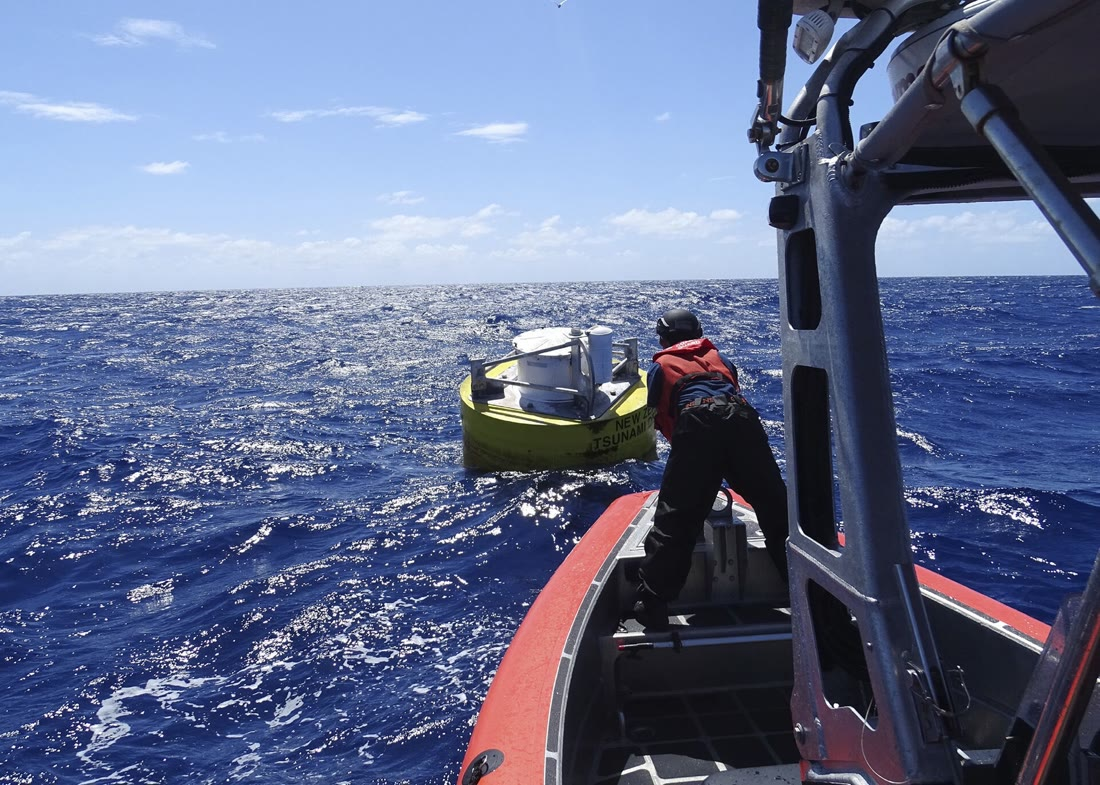
\includegraphics[width=\linewidth]{images/book1/g9-dart-buoy.jpg}
\end{minipage}\hfill
\begin{minipage}[c]{0.56\linewidth}\raggedright
{\small Een bemanningslid van een schip van de Amerikaanse kustwacht
inspecteert een tsunamiwaarschuwingsboei in de Stille \omterm{def:g2:water-on-earth:ocean}{Oceaan}, in november
2021. De boei drijft boven een drukmeter op de zeebodem, duizenden meters
lager. U.S. Coast Guard (publiek domein, via Wikimedia Commons).}
\end{minipage}
% ledger: commons:dart-buoy
\label{fig:g9:natural-risks:buoy}
\end{omfigure}

\begin{history}[Een netwerk van boeien]
In 2001 was de eerste reeks van zes zulke stations in de Stille \omterm{def:g2:water-on-earth:ocean}{Oceaan}
klaar. Na de \omterm{def:g7:earthquakes:tsunami}{tsunami} van december 2004, die de \omterm{def:g1:landscapes-around-us:water}{kusten} van de Indische
\omterm{def:g2:water-on-earth:ocean}{Oceaan} bereikte terwijl er geen waarschuwingssysteem was
(\cref{ch:g7:earthquakes}), groeide het netwerk: in maart 2008 waren er
39 stations.
\end{history}
% ledger: ndbc:dart

Een waarschuwing redt alleen levens als ze mensen bereikt die weten wat ze
ermee moeten doen: de routes naar hoger gelegen grond zijn aangegeven en
geoefend, het noodpakket staat klaar, scholen houden oefeningen. In Armero
was het gevaar bekend en was de \omterm{def:g2:drawing-to-map:map}{kaart} getekend; de waarschuwing heeft de
stad nooit bereikt.
% ledger: ready:kit, usgs:armero

\section{Oefeningen}

\begin{exercise}[$\star$]\label{exo:g9:natural-risks:1}
Gevaar of \omterm{def:g9:natural-risks:vulnerability}{kwetsbaarheid}? (a) Een \omterm{def:g1:landscapes-around-us:water}{rivier} die bijna elk voorjaar
overstroomt. (b) Een dorp zonder waarschuwingssysteem. (c) Zware huizen
van baksteen zonder skelet. (d) Een zware \omterm{def:g4:volcanoes-earthquakes-first-look:earthquake}{aardbeving} op een nabije \omterm{def:g7:earthquakes:fault}{breuk}.
(e) Een stad gebouwd aan de \omterm{def:g5:water-shapes-the-land:source-mouth}{monding} van een \omterm{def:g1:landscapes-around-us:landform}{dal} waar al eerder
modderstromen door zijn gekomen.
\end{exercise}

\begin{exercise}[$\star$]\label{exo:g9:natural-risks:2}
Waar of niet waar? Verbeter de onware zinnen. (a) Een \omterm{def:g5:natural-hazards:hazard}{natuurgevaar} op een
plaats waar niemand woont, is een hoog \omterm{def:g9:natural-risks:risk}{risico}. (b) \omterm{def:g9:natural-risks:prevention}{Preventie} kan de
\omterm{def:g9:natural-risks:vulnerability}{kwetsbaarheid} van een stad verlagen. (c) Een \omterm{def:g9:natural-risks:hazard-map}{gevarenkaart} toont waar een
gevaar kan toeslaan. (d) Een goed waarschuwingssysteem maakt een \omterm{def:g4:volcanoes-earthquakes-first-look:volcano}{vulkaan}
minder gevaarlijk.
\end{exercise}

\begin{exercise}[$\star$]\label{exo:g9:natural-risks:3}
Zeg voor elk gevaar of het dagen of uren van tevoren kan worden voorspeld:
(a) een \omterm{def:g5:natural-hazards:storm}{storm}; (b) een \omterm{def:g5:water-shapes-the-land:flood}{overstroming} na zware \omterm{def:g4:clouds-rain-snow:precipitation}{regen}; (c) een \omterm{def:g4:volcanoes-earthquakes-first-look:earthquake}{aardbeving};
(d) de aankomst van een \omterm{def:g7:earthquakes:tsunami}{tsunami} op een \omterm{def:g1:landscapes-around-us:water}{kust} ver van waar hij ontstond.
\end{exercise}

\begin{exercise}[$\star$]\label{exo:g9:natural-risks:4}
% ledger: usgs:hvo-toolkit
Gebruik de tekening van een bewaakte \omterm{def:g4:volcanoes-earthquakes-first-look:volcano}{vulkaan}. Wat meet elk instrument, en
naar welk waarschuwingssignaal van een \omterm{def:g4:volcanoes-earthquakes-first-look:eruption}{uitbarsting} kijkt het? (a) Een
\omterm{def:g7:earthquakes:seismometer}{seismometer}. (b) Een hellingmeter. (c) Een gps-ontvanger. (d) Een
gasmeter.
\end{exercise}

\begin{exercise}[$\star\star$]\label{exo:g9:natural-risks:5}
% ledger: usgs:armero
In 1985 bereikten de modderstromen van de Nevado del Ruiz Armero,
\qty{45}{km} verderop, ongeveer twee uur na de \omterm{def:g4:volcanoes-earthquakes-first-look:eruption}{uitbarsting}. (a) Wat was hun
gemiddelde snelheid, in kilometer per uur? (b) Iemand loopt ongeveer
\qty{4}{km/h}. Hoe ver hadden de mensen in twee uur kunnen lopen?
(c) Waarom vertrokken ze niet? (d) Noem twee dingen die hen hadden kunnen
redden.
\end{exercise}

\begin{exercise}[$\star\star$]\label{exo:g9:natural-risks:6}
% ledger: (invented region: figdata/grade-9/flood_zone.py)
Gebruik de \omterm{def:g2:drawing-to-map:map}{kaart} van de overstromingszones van de Varden Hills.
(a) Welke \omterm{def:g5:water-shapes-the-land:flood}{overstroming} bedekt de breedste strook? (b) Meet met het rooster
van de \omterm{def:g2:drawing-to-map:map}{kaart} de breedte van elke zone dwars door het \omterm{def:g1:landscapes-around-us:landform}{dal}, op
\qty{5}{km} oost. (c) Een schuur staat op grond die \qty{6}{m} boven de
\omterm{def:g1:landscapes-around-us:water}{rivier} ligt.
Welke van de drie \omterm{def:g5:water-shapes-the-land:flood}{overstromingen} bereiken haar? (d) Waarom komt de
\omterm{def:g5:water-shapes-the-land:flood}{overstroming} van \qty{2}{m} boven de \omterm{def:g1:landscapes-around-us:water}{rivier} het vaakst voor?
\end{exercise}

\begin{exercise}[$\star\star$]\label{exo:g9:natural-risks:7}
Plaats elke situatie in het risicorooster (klein of groot gevaar, kleine
of grote \omterm{def:g9:natural-risks:vulnerability}{kwetsbaarheid}) en zeg of het \omterm{def:g9:natural-risks:risk}{risico} laag, matig of hoog is.
(a) Stevige gebouwen en oefeningen in een stad op een actieve \omterm{def:g7:earthquakes:fault}{breuk}.
(b) Een camping op de \omterm{def:g5:water-shapes-the-land:flood}{overstromingsvlakte} van een \omterm{def:g1:landscapes-around-us:water}{rivier} die zelden
overstroomt. (c) Een dorp van zwakke huizen aan de voet van een actieve
\omterm{def:g4:volcanoes-earthquakes-first-look:volcano}{vulkaan}, zonder observatorium. (d) Een stad op een heuveltop ver van elke
\omterm{def:g7:earthquakes:fault}{breuk}, \omterm{def:g1:landscapes-around-us:water}{rivier} of \omterm{def:g4:volcanoes-earthquakes-first-look:volcano}{vulkaan}.
\end{exercise}

\begin{exercise}[$\star\star$]\label{exo:g9:natural-risks:8}
% ledger: iris:better-wall, explo:base-isolation
Drie scholen worden op dezelfde grond gebouwd. School A is een skelet van
palen en balken met bakstenen muren ertussen; school B heeft hetzelfde
skelet met diagonale schoren en twee schijfwanden; school C heeft het
skelet van B, op isolatoren. (a) Rangschik ze van de veiligste tot de
minst veilige bij een \omterm{def:g4:volcanoes-earthquakes-first-look:earthquake}{aardbeving}. (b) Leg uit wat de schoren doen.
(c) Leg uit wat de isolatoren doen.
\end{exercise}

\begin{exercise}[$\star\star$]\label{exo:g9:natural-risks:9}
% ledger: fema:flood-zones
Een overstromingskaart toont de honderdjaarsoverstroming, die elk jaar
een kans van 1 op 100 heeft om te worden bereikt of overschreden.
(a) Schrijf deze kans als percentage. (b) Een buurman zegt: ``De
honderdjaarsoverstroming kwam vorig jaar, dus we zijn 99 jaar veilig.''
Wat klopt er niet? (c) Hoeveel zulke \omterm{def:g5:water-shapes-the-land:flood}{overstromingen} zouden er gemiddeld
in 300 jaar komen?
\end{exercise}

\begin{exercise}[$\star\star$]\label{exo:g9:natural-risks:10}
% ledger: ndbc:dart, nws:tsunami-speed
Een station voor tsunamiwaarschuwing leest elke \qty{15}{s} de druk op de
zeebodem af. (a) Hoeveel metingen doet het in één uur? (b) In één jaar van
365 dagen? Schrijf het antwoord in de wetenschappelijke notatie. (c) Een
\omterm{def:g7:earthquakes:tsunami}{tsunami} steekt de diepe \omterm{def:g2:water-on-earth:ocean}{oceaan} over met ongeveer \qty{800}{km/h}. Hoe lang
doet hij erover om een \omterm{def:g1:landscapes-around-us:water}{kust} op \qty{2400}{km} afstand te bereiken?
(d) Waarom is die tijd belangrijk?
\end{exercise}

\begin{exercise}[$\star\star\star$]\label{exo:g9:natural-risks:11}
% ledger: ready:kit
Een gezin van vier stelt een noodpakket samen met water voor 3 dagen, met
ongeveer \qty{3.8}{L} per persoon per dag, om te drinken en te wassen.
(a) Hoeveel liter water hebben ze nodig? (b) Hoeveel flessen van
\qty{1.5}{L} is dat? (c) Noem vier andere dingen in het pakket, en zeg
waarom elk ervan nuttig is. (d) Waarom ligt het pakket bij de deur?
\end{exercise}

\begin{exercise}[$\star\star\star$]\label{exo:g9:natural-risks:12}
% ledger: usgs:armero, usgs:hvo-toolkit
Een stad ligt naast een \omterm{def:g1:landscapes-around-us:water}{rivier}, aan de \omterm{def:g5:water-shapes-the-land:source-mouth}{monding} van een \omterm{def:g1:landscapes-around-us:landform}{dal} dat van een
besneeuwde \omterm{def:g4:volcanoes-earthquakes-first-look:volcano}{vulkaan} naar beneden komt. Onder haar straten liggen oude
afzettingen van modderstromen. De \omterm{def:g4:volcanoes-earthquakes-first-look:volcano}{vulkaan} is begonnen te schudden met
kleine \omterm{def:g4:volcanoes-earthquakes-first-look:earthquake}{aardbevingen}. Schrijf een preventieplan van vijf punten voor de
stad. Zeg bij elk punt of het aan de kant van het gevaar werkt (het gevaar
kennen en in de gaten houden) of aan de kant van de \omterm{def:g9:natural-risks:vulnerability}{kwetsbaarheid}.
\end{exercise}

\section{Probleem: Waar komt de nieuwe school?}

\begin{problem}[{Weekendprobleem --- een nieuwe school wordt op de kaart
van de Varden Hills geplaatst, weg van overstromingen, steile hellingen en
de breuk; het eindantwoord is het aantal huizen in de overstromingszone}]
\label{pb:g9:natural-risks:1}
% ledger: (invented region: figdata/grade-9/flood_zone.py: sites A, B, C; 17 of 28 houses in the 5 m zone)
Het dorp van de Varden Hills heeft een nieuwe school nodig, en er worden
drie plaatsen aangeboden: A, B en C, op de \omterm{def:g2:drawing-to-map:map}{kaart} hieronder. De
overstromingszone die op de \omterm{def:g2:drawing-to-map:map}{kaart} is gearceerd, is alle grond die minder
dan \qty{5}{m} boven de \omterm{def:g1:landscapes-around-us:water}{rivier} ligt en die een grote \omterm{def:g5:water-shapes-the-land:flood}{overstroming} zou
bedekken. De tabel geeft voor elke plaats de hoogte van de grond, het peil
van de \omterm{def:g1:landscapes-around-us:water}{rivier} ernaast, en hoeveel de grond stijgt over \qty{200}{m}
horizontaal gemeten dwars over de helling.

\begin{center}
{\small
\begin{tabular}{|c|c|c|c|}
\hline
plaats & hoogte van de grond & peil van de \omterm{def:g1:landscapes-around-us:water}{rivier} ernaast & stijging van de grond over \qty{200}{m} \\
\hline
A & \qty{137}{m} & \qty{137}{m} & \qty{1.4}{m} \\
B & \qty{276}{m} & \qty{126}{m} & \qty{83}{m} \\
C & \qty{236}{m} & \qty{143}{m} & \qty{20}{m} \\
\hline
\end{tabular}}
\end{center}

\begin{omfigure}
\begin{tikzpicture}
\begin{axis}[axis equal image, xmin=3.5, xmax=7, ymin=2.7, ymax=5.5, width=11.5cm,
  enlargelimits=false, tick label style={font=\scriptsize}, xlabel={oost (km)},
  ylabel={noord (km)}, label style={font=\small}, xtick={3.5,4,...,7}, ytick={3,3.5,...,5.5}]
\addplot[contour] table {figdata/out/grade-9-flood_zone-contours.dat};
\addplot[index contour] table {figdata/out/grade-9-flood_zone-index.dat};
\addplot[fill=blue!25, draw=blue!50, line width=0.3pt] table {figdata/out/grade-9-flood_zone-zone.dat} -- cycle;
\addplot[only marks, mark=none, point meta=explicit symbolic, nodes near coords,
  nodes near coords align={center}, nodes near coords style={font=\tiny, fill=white, inner sep=0.6pt, text=omContour}]
  table[meta=z] {figdata/out/grade-9-flood_zone-index-lab.dat};
\addplot[river] table {figdata/out/grade-9-flood_zone-river.dat};
\addplot[fault] table {figdata/out/shared-region-fault.dat};
\addplot[only marks, mark=square*, mark size=1.5pt, mark options={fill=black}] table {figdata/out/grade-9-flood_zone-houses-in.dat};
\addplot[only marks, mark=square*, mark size=1.5pt, mark options={fill=black}] table {figdata/out/grade-9-flood_zone-houses-out.dat};
\addplot[only marks, mark=*, mark size=2.6pt, mark options={fill=omWarm, draw=black}, point meta=explicit symbolic,
  nodes near coords, nodes near coords align={anchor=south west},
  nodes near coords style={font=\small\bfseries, fill=white, inner sep=1pt, xshift=2.5pt, yshift=2.5pt}]
  table[meta=name] {figdata/out/grade-9-flood_zone-sites.dat};
\node[font=\footnotesize, fill=white, inner sep=1pt, anchor=west] at (axis cs:6.42,5.05) {breuk};
\coordinate (na) at (axis cs:3.7,4.75);
\fill[black] (axis cs:5.8,2.85) rectangle (axis cs:5.925,2.9);
\fill[white] (axis cs:5.925,2.85) rectangle (axis cs:6.05,2.9);
\fill[black] (axis cs:6.05,2.85) rectangle (axis cs:6.175,2.9);
\fill[white] (axis cs:6.175,2.85) rectangle (axis cs:6.3,2.9);
\draw[black, line width=0.4pt] (axis cs:5.8,2.85) rectangle (axis cs:6.3,2.9);
\node[font=\footnotesize, above, inner sep=1.5pt, fill=white] at (axis cs:6.05,2.9) {\qty{500}{m}};
\end{axis}
\fill[white, opacity=0.85] ($(na)+(-0.35,-0.1)$) rectangle ($(na)+(0.35,1.45)$);
\pic at (na) {northarrow};
\end{tikzpicture}

{\small Het dorp, de drie plaatsen voor de school en de overstromingszone
(gearceerd), op de \omterm{def:g2:drawing-to-map:map}{kaart} van de Varden Hills (dunne lijnen van gelijke
hoogte om de \qty{10}{m}). Elk zwart vierkantje is een huis. De dikke
zwarte lijn is een \omterm{def:g7:earthquakes:fault}{breuk}.}
\label{fig:g9:natural-risks:school-map}
\end{omfigure}

\noindent\textbf{Deel I --- De overstromingszone.}\par\nopagebreak
\begin{enumerate}[beginpenalty=10000]
  \item Zeg met de rivierpeilen van de tabel in welke richting de \omterm{def:g1:landscapes-around-us:water}{rivier}
        stroomt.
  \item Bereken de hoogte van elke plaats boven de \omterm{def:g1:landscapes-around-us:water}{rivier} ernaast.
  \item Welke van de drie plaatsen ligt in de overstromingszone?
  \item Meet met de schaalbalk de breedte van de overstromingszone dwars
        door het \omterm{def:g1:landscapes-around-us:landform}{dal}, bij plaats A.
\end{enumerate}

\noindent\textbf{Deel II --- De hellingen en de breuk.}\par\nopagebreak
\begin{enumerate}[resume, beginpenalty=10000]
  \item Een helling in procent is de stijging van de grond per
        \qty{100}{m} horizontaal gemeten. Bereken de helling bij elke
        plaats.
  \item Welke plaats zou aan een \omterm{def:g5:natural-hazards:landslide}{aardverschuiving} blootstaan? Leg uit.
  \item Schat met de schaalbalk de afstand van elke plaats tot de \omterm{def:g7:earthquakes:fault}{breuk}.
  \item Stel dat de \omterm{def:g7:earthquakes:fault}{breuk} nog kan verschuiven. Waarom is de grond er recht
        bovenop een slechte plaats voor een school?
\end{enumerate}

\noindent\textbf{Deel III --- Kiezen.}\par\nopagebreak
\begin{enumerate}[resume, beginpenalty=10000]
  \item Teken een tabel met één rij per plaats en drie kolommen: in de
        overstromingszone? steile helling? op de \omterm{def:g7:earthquakes:fault}{breuk}? Vul hem in met ja
        of nee.
  \item Welke plaats zou jij kiezen? Verantwoord je keuze met de tabel.
  \item De gekozen plaats ligt nog steeds in een gebied waar de grond kan
        schudden. Noem twee manieren om de school te bouwen, en één
        gewoonte van de leerlingen, die haar \omterm{def:g9:natural-risks:vulnerability}{kwetsbaarheid} verlagen.
  \item De school zal ook dienen als schuilplaats bij \omterm{def:g5:water-shapes-the-land:flood}{overstromingen}. Tel
        de huizen van het dorp die in de overstromingszone staan. Welk deel
        van alle huizen is dat?
\end{enumerate}
\end{problem}
